\documentclass[handout]{mcs}

\begin{document}

\inclassproblems{2, Mon.}

%%%%%%%%%%%%%%%%%%%%%%%%%%%%%%%%%%%%%%%%%%%%%%%%%%%%%%%%%%%%%%%%%%%%%
% Problems start here
%%%%%%%%%%%%%%%%%%%%%%%%%%%%%%%%%%%%%%%%%%%%%%%%%%%%%%%%%%%%%%%%%%%%%

\pinput{CP_truth_table_for_distributive_law}
\insolutions{\newpage}
\pinput{CP_file_system_functioning_normally}
%\pinput{CP_valid_vs_satisfiable}
\pinput{CP_differentiable_implies_continuous}
\pinput{CP_binary_adder_logic}
%\pinput{CP_faster_adder_logic}


\instatements{\newpage}
%\section*{Appendix}
\section*{The Propositional Operations}

\[
\begin{array}{c|c}
P & \QNOT P \\ \hline
\true & \false \\
\false & \true \\
\end{array}
\]

\[
\begin{array}{cc|c}
P & Q & P \QAND Q \\ \hline
\true & \true & \true \\
\true & \false & \false \\
\false & \true & \false \\
\false & \false & \false
\end{array}
\]


\[
\begin{array}{cc|c}
P & Q & P \QOR Q \\ \hline
\true & \true & \true \\
\true & \false & \true \\
\false & \true & \true \\
\false & \false & \false
\end{array}
\]

\[
\begin{array}{cc|c}
P & Q & P \QXOR Q \\ \hline
\true & \true & \false \\
\true & \false & \true \\
\false & \true & \true \\
\false & \false & \false
\end{array}
\]

\[
\begin{array}{cc|c}
    P  &   Q    & P \QIMP Q \\ \hline
\true  & \true  & \true \\
\true  & \false & \false \\
\false & \true  & \true \\
\false & \false & \true  
\end{array}
\]

\[
\begin{array}{cc|c}
P & Q & P \QIFF Q \\ \hline
\true & \true & \true \\
\true & \false & \false \\
\false & \true & \false \\
\false & \false & \true
\end{array}
\]

\begin{figure}[htbp]
%\centering 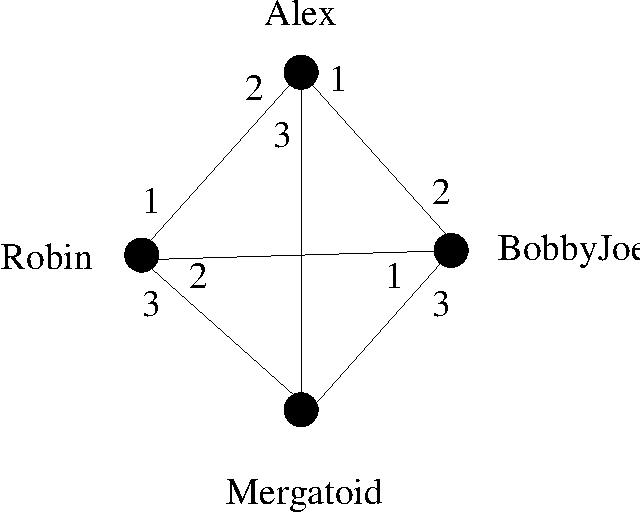
\includegraphics[height=2.3in]{figures/loveTriangle.pdf}
%\includegraphics{latex-macros/figures/add1-circuit-diagram.pdf}
\includegraphics[height=9in]{add1-circuit-diagram.pdf}
\caption{Structure of a Double-size Add1 Module.}
\label{fig:add1}
\end{figure}

%%%%%%%%%%%%%%%%%%%%%%%%%%%%%%%%%%%%%%%%%%%%%%%%%%%%%%%%%%%%%%%%%%%%%
% Problems end here
%%%%%%%%%%%%%%%%%%%%%%%%%%%%%%%%%%%%%%%%%%%%%%%%%%%%%%%%%%%%%%%%%%%%%
\end{document}

